% =============================================================================
%  fig_key_results.tex  — journal compact two-panel figure
%  Left : Phase-A estimated waveform decomposition (model vs measured concept)
%  Right: Security margin comparison (fixed vs adaptive pickup on I_rms curve)
%  Standalone, compiles with pdflatex
% =============================================================================
\documentclass[tikz, border=5pt]{standalone}
\usepackage{tikz}
\usepackage{pgfplots}
\pgfplotsset{compat=1.18}
\usepackage{amsmath}
\usetikzlibrary{arrows.meta, positioning, calc, decorations.pathreplacing}

% Palette (greyscale-safe, IEEE colour-blind safe)
\definecolor{measC}   {RGB}{ 31, 119, 180}   % measured — blue
\definecolor{modelC}  {RGB}{214,  39,  40}   % model — red
\definecolor{envC}    {RGB}{255, 127,  14}   % envelope — orange
\definecolor{dcC}     {RGB}{ 44, 160,  44}   % DC — green
\definecolor{fixC}    {RGB}{ 31, 119, 180}   % fixed pickup
\definecolor{adaptC}  {RGB}{214,  39,  40}   % adaptive pickup

\begin{document}
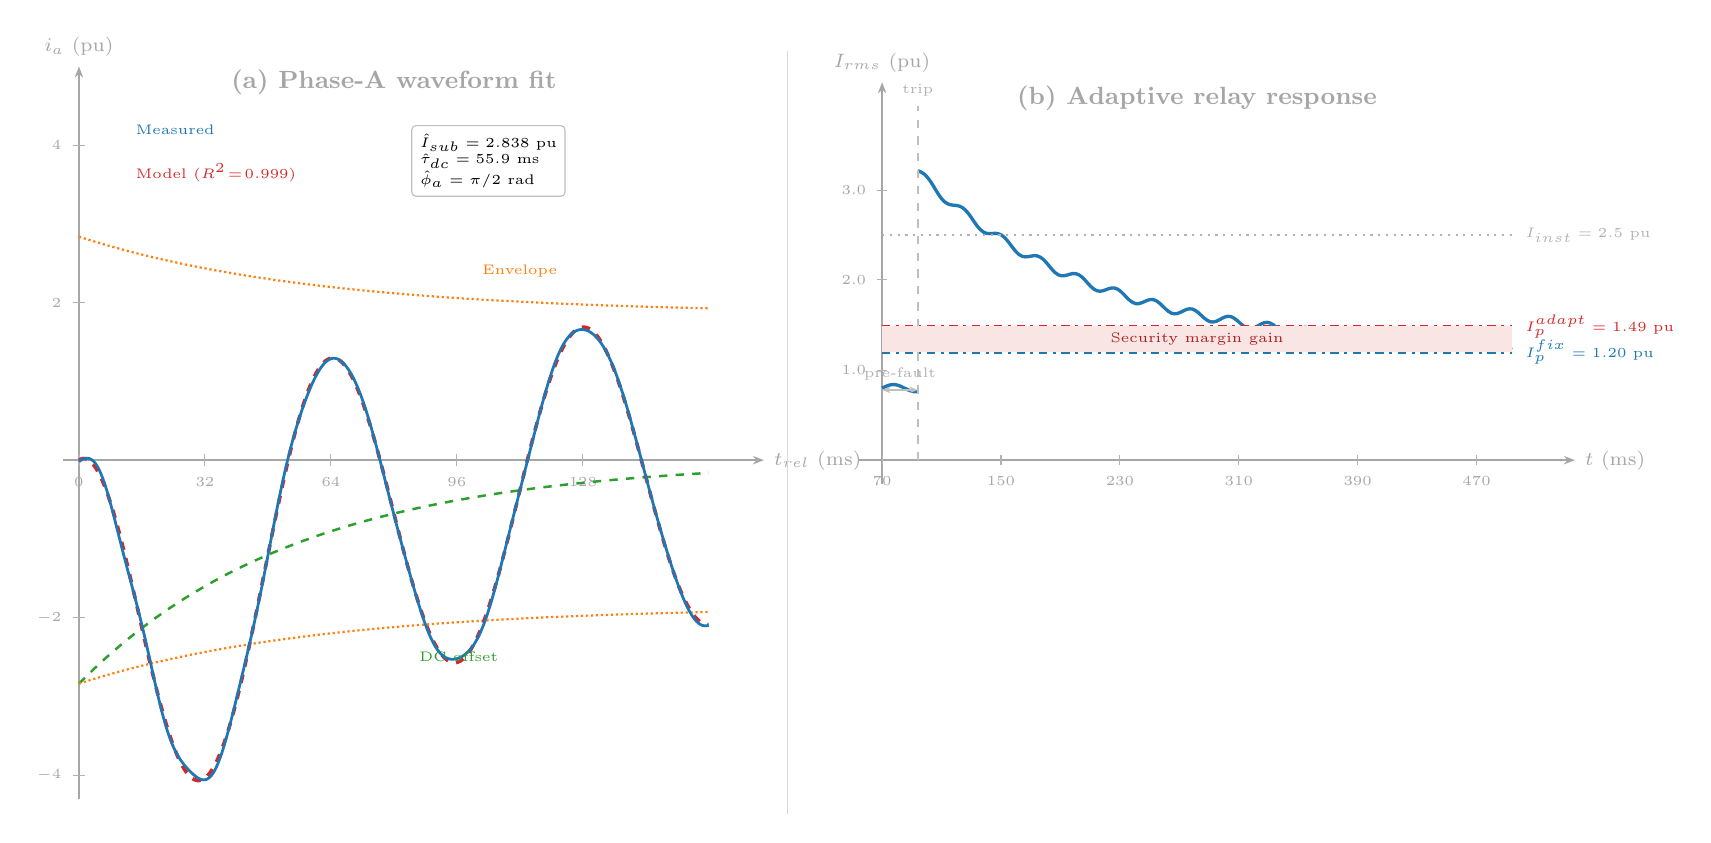
\begin{tikzpicture}

% ============================================================
% PANEL A — Phase-A waveform: measured vs fitted, with DC
% ============================================================
\begin{scope}

% Axes
\draw[-{Stealth[length=4pt]}, gray!70, line width=0.7pt]
  (-0.2, 0) -- (8.7, 0) node[right, font=\scriptsize] {$t_{rel}$ (ms)};
\draw[-{Stealth[length=4pt]}, gray!70, line width=0.7pt]
  (0, -4.3) -- (0, 5.0) node[above, font=\scriptsize] {$i_a$ (pu)};

% Axis ticks
\foreach \x/\lbl in {0/0, 1.6/32, 3.2/64, 4.8/96, 6.4/128}{
  \draw[gray!60, line width=0.4pt] (\x, -0.08) -- (\x, 0.08);
  \node[below, font=\tiny, gray!70] at (\x, -0.1) {\lbl};
}
\foreach \y/\lbl in {-4/$-4$, -2/$-2$, 2/$2$, 4/$4$}{
  \draw[gray!60, line width=0.4pt] (-0.08, \y) -- (0.08, \y);
  \node[left, font=\tiny, gray!70] at (-0.1, \y) {\lbl};
}

% Normalisation: x-axis 0..8cm = 0..160ms, y-axis scale: 1cm=1pu
% Parameters: I_sub=2.838, I_ss=1.858, tau_ac=60.6ms, tau_dc=55.9ms, phi=pi/2
\def\om{3.14159}   % half-period = 1 cycle width = 3.2cm (20ms*160)
\def\Iss{1.858}
\def\Isub{2.838}
\def\tauac{3.03}   % 60.6ms / (160ms/8cm) = 3.03cm
\def\taudc{2.795}  % 55.9ms / 20ms * ... = 55.9/160*8 = 2.795cm

% DC offset (green) — drawn first so other lines go over it
\draw[dcC, line width=0.9pt, dashed]
  plot[domain=0:8, samples=80, smooth]
  (\x, {-\Isub * exp(-\x/\taudc)});

% AC envelope upper (orange dashed)
\draw[envC, line width=0.8pt, densely dotted]
  plot[domain=0:8, samples=60, smooth]
  (\x, {\Iss + (\Isub-\Iss)*exp(-\x/\tauac)});
\draw[envC, line width=0.8pt, densely dotted]
  plot[domain=0:8, samples=60, smooth]
  (\x, {-(\Iss + (\Isub-\Iss)*exp(-\x/\tauac))});

% Model current: i_a = envelope*sin(wt+pi/2) + DC*exp(-t/tau_dc)
\draw[modelC, line width=1.3pt, dashed]
  plot[domain=0:8, samples=300, smooth]
  (\x, {(\Iss+(\Isub-\Iss)*exp(-\x/\tauac)) * sin(deg(\om*\x/1.6)+90)
        + (-\Isub*exp(-\x/\taudc))});

% Measured current (slightly perturbed — representative noise)
\draw[measC, line width=1.0pt]
  plot[domain=0:8, samples=300, smooth]
  (\x, {(\Iss+(\Isub-\Iss)*exp(-\x/\tauac)+0.04*sin(deg(7.3*\x+1.2)))
        * sin(deg(\om*\x/1.6)+90+0.015*sin(deg(5*\x)))
        + (-\Isub*exp(-\x/\taudc))*(1+0.02*cos(deg(11*\x)))});

% Labels
\node[right, font=\tiny, measC] at (0.6,  4.2) {Measured};
\node[right, font=\tiny, modelC] at (0.6, 3.65) {Model ($R^2\!=\!0.999$)};
\node[right, font=\tiny, envC]  at (5.0,  2.4) {Envelope};
\node[right, font=\tiny, dcC]   at (4.2, -2.5) {DC offset};

% Annotation box
\node[draw=gray!50, fill=white, rounded corners=1.5pt, inner sep=3pt,
      font=\tiny, align=left] at (5.2, 3.8)
{$\hat{I}_{sub}=2.838$ pu\\$\hat{\tau}_{dc}=55.9$ ms\\$\hat{\phi}_a=\pi/2$ rad};

% Panel label
\node[font=\small\bfseries, gray!70] at (4.0, 4.8) {(a) Phase-A waveform fit};

\end{scope}

% ============================================================
% PANEL B — Relay I_rms + security margin (right of panel A)
% ============================================================
\begin{scope}[xshift=10.2cm]

% Axes
\draw[-{Stealth[length=4pt]}, gray!70, line width=0.7pt]
  (-0.3,0) -- (8.8,0) node[right, font=\scriptsize]{$t$ (ms)};
\draw[-{Stealth[length=4pt]}, gray!70, line width=0.7pt]
  (0,-0.3) -- (0,4.8) node[above, font=\scriptsize]{$I_{rms}$ (pu)};

% Axis ticks — x: 70..600ms mapped to 0..8cm (530ms range)
\foreach \x/\lbl in {0/70, 1.51/150, 3.02/230, 4.53/310, 6.04/390, 7.55/470}{
  \draw[gray!60, line width=0.4pt] (\x, -0.06) -- (\x, 0.06);
  \node[below, font=\tiny, gray!70] at (\x, -0.08) {\lbl};
}
% y: 0..3.5 pu mapped to 0..4 cm
\foreach \y/\lbl in {1.14/1.0, 2.29/2.0, 3.43/3.0}{
  \draw[gray!60, line width=0.4pt] (-0.06, \y) -- (0.06, \y);
  \node[left, font=\tiny, gray!70] at (-0.08, \y) {\lbl};
}

% I_rms: rises sharply at t=100ms (x≈0.23), peaks ~3.2pu, decays
% t=70..600ms → x = (t-70)/530*8
% I_rms(t) ≈ (0.8 + 2.4*H(t-100)*exp(-(t-100)/80)) pu, scaled to cm
% Scale: 1cm = 0.875pu (4cm = 3.5pu)
\def\sc{1.143}    % cm per pu
\def\t0x{0.453}   % x-coord of t=100ms  (100-70)/530*8 = 0.453

\draw[measC, line width=1.2pt]
  plot[domain=0:\t0x, samples=20, smooth]
  (\x, {0.8*\sc * (1 + 0.05*sin(deg(11*\x)))});

% Post-fault I_rms: peak then exponential decay
\draw[measC, line width=1.2pt]
  plot[domain=\t0x:8, samples=200, smooth]
  (\x, {\sc * (1.2 + 2.0*exp(-((\x-\t0x)*530/8)/150)
        + 0.05*sin(deg(13*(\x-\t0x)+0.3)))});

% Fixed pickup threshold line
\draw[fixC, line width=1.1pt, dash dot]
  (0, {1.200*\sc}) -- (8, {1.200*\sc});
\node[right, font=\tiny, fixC] at (8.05, {1.200*\sc}) {$I_p^{fix}=1.20$ pu};

% Adaptive pickup threshold line
\draw[adaptC, line width=1.1pt, dash dot]
  (0, {1.487*\sc}) -- (8, {1.487*\sc});
\node[right, font=\tiny, adaptC] at (8.05, {1.487*\sc}) {$I_p^{adapt}=1.49$ pu};

% Instantaneous threshold
\draw[gray!60, line width=0.8pt, dotted]
  (0, {2.500*\sc}) -- (8, {2.500*\sc});
\node[right, font=\tiny, gray!60] at (8.05, {2.500*\sc}) {$I_{inst}=2.5$ pu};

% Trip marker
\draw[gray!50, line width=0.8pt, dashed]
  (\t0x, 0) -- (\t0x, 4.5);
\node[above, font=\tiny, gray!60] at (\t0x, 4.5) {trip};

% Security margin shading (between fixed and adaptive pickup)
\fill[adaptC!12]
  (0, {1.200*\sc}) rectangle (8, {1.487*\sc});
\node[font=\tiny, adaptC!80!black] at (4.0, {(1.200+1.487)/2*\sc})
  {Security margin gain};

% Pre-fault zone arrow
\draw[{Stealth[length=3pt]}-{Stealth[length=3pt]}, gray!50, line width=0.5pt]
  (0, {0.78*\sc}) -- (\t0x, {0.78*\sc});
\node[font=\tiny, gray!60, above] at (\t0x/2, {0.78*\sc}) {pre-fault};

% Panel label
\node[font=\small\bfseries, gray!70] at (4.0, 4.6) {(b) Adaptive relay response};

\end{scope}

% ============================================================
% Separator rule between panels
% ============================================================
\draw[gray!30, line width=0.5pt] (9.0, -4.5) -- (9.0, 5.2);

\end{tikzpicture}
\end{document}
